% This is samplepaper.tex, a sample chapter demonstrating the
% LLNCS macro package for Springer Computer Science proceedings;
% Version 2.21 of 2022/01/12
%
\documentclass[runningheads]{llncs}
%
\usepackage[T1]{fontenc}
% T1 fonts will be used to generate the final print and online PDFs,
% so please use T1 fonts in your manuscript whenever possible.
% Other font encondings may result in incorrect characters.
%
\usepackage[utf8]{inputenc}
\usepackage{url}
\usepackage{graphicx}
\usepackage{hyperref}
\usepackage{listings}
\usepackage{amsmath}
\usepackage{amssymb}
\usepackage[inline]{enumitem}
\usepackage{makecell}
\usepackage{tabularx}
% Used for displaying a sample figure. If possible, figure files should
% be included in EPS format.
%
% If you use the hyperref package, please uncomment the following two lines
% to display URLs in blue roman font according to Springer's eBook style:
%\usepackage{color}
%\renewcommand\UrlFont{\color{blue}\rmfamily}
%\urlstyle{rm}
%

\begin{document}
    \setlist[enumerate]{noitemsep, topsep=0pt}
%
%    \title{{\fontsize{14}{16}\selectfont Client-Driven Offline-First RDF 1.2 using OR-Sets}}

    \title{Demonstration of Composable SPARQL Parsing and Query Execution with Traqula and Comunica}
%
%\titlerunning{Abbreviated paper title}
% If the paper title is too long for the running head, you can set
% an abbreviated paper title here
%
    \author{Jitse De Smet\inst{1}\orcidID{0009-0002-6513-5013} \and
    Ruben Taelman\inst{1}\orcidID{0000-0001-5118-256X}}
%
    \authorrunning{J. De Smet and R. Taelman}
% First names are abbreviated in the running head.
% If there are more than two authors, 'et al.' is used.
%
    \institute{IDLab, Department of Electronics and Information Systems, Ghent University – imec.
    \email{\{firstname\}.\{lastname\}@ugent.be}}
%
    \maketitle              % typeset the header of the contribution
%
    \begin{abstract}
        Linked Data and SPARQL are becoming increasingly diverse, with engines
        supporting different dialects and extensions. With SPARQL 1.2 nearing
        completion and its planned maintenance mode, this diversity is expected
        to grow. There is a growing need for language tools that can handle
        multiple versions and dialects in a unified way. In response, we
        introduced Traqula, a modular framework for parsing, generating, and
        transforming queries, allowing components to be created and adapted
        incrementally. This paper showcases a web client that brings together
        Traqula and the modular Comunica query engine, enabling users to
        experiment with queries across multiple parser and engine variants while
        interactively visualizing their configuration, illustrating the power of
        modularity for both language tools and query engines.



        \keywords{SPARQL \and
                  parser \and
                  query engine \and
                  modularity}

        \textbf{Video}: \href{https://youtu.be/7VFJGvxbRsI}{https://youtu.be/7VFJGvxbRsI} \\
        \textbf{Online Demo}: \href{https://compose-parser-engine.demo.jitsedesmet.be/}{https://compose-parser-engine.demo.jitsedesmet.be/} \\
        \textbf{Canonical version}: \href{https://2026-eswc-demo.jitsedesmet.be/}{https://2026-eswc-demo.jitsedesmet.be/}
    \end{abstract}
%
%
%


    \section{Introduction}
    \label{introduction}

    Linked Data on the Web exists in diverse forms~\cite{spec:sparqlprot,tpf,smartkg},
    enabling the RDF model to support varied environments and querying
    algorithms across single or multiple sources. The modular query engine
    Comunica~\cite{comunica} was introduced to unify querying
    over these different RDF interfaces while supporting multiple data
    access and processing algorithms. It's modular architecture has proven
    effective, enabling \emph{sustainable} maintenance of a
    SPARQL 1.1~\cite{spec:sparqllang} query engine that
    supports many dataset types and execution strategies. However, Comunica
    has so far been limited to processing basic SPARQL 1.1 queries and
    - through conversion step - a subset of GraphQL~\cite{graphql-ld}.

    This limitation was not arbitrary, but technical. The software
    responsible for parsing and generating SPARQL queries- transforming query
    strings to and from SPARQL algebra- was implemented as a large monolithic
    component. Extending this component would require either:
    \begin{enumerate}
      \item maintaining a long-term fork
      \item introducing language extensions that change the behaviour of the upstream parser beyond SPARQL 1.1, or
      \item preserving backward compatibility through extensive conditional logic, ultimately harming maintainability.
    \end{enumerate}

    At the same time, SPARQL itself has evolved heterogeneously. Different engines implement their own
    dialects~\cite{geosparql,tsparql} and extensions: Virtuoso supports full
    text search~\cite{virtuoso-full-text-search}, Jena supports
    constructing quads~\cite{jena-construct-quad}, and oxigraph supports
    the built-in Adjust~\cite{sparql-adjust,oxigraph-adjust}. This diversity is expected to increase further
    with the emergence of SPARQL 1.2~\cite{sparql-1-2} and
    its planned \href{https://github.com/w3c/sparql-dev/issues/32\#issuecomment-2621209920}{maintenance
    mode}~\cite{rdf12-charter}.

    To address these challenges, we developed Traqula~\cite{traqula}, a toolkit for parsing,
    generating, and transforming query languages. As described in our accepted ESWC 2026 resource paper~\cite{traqula}, Traqula
    enables incremental modification of existing SPARQL 1.1 and SPARQL 1.2
    parsing setups while remaining generic enough to support future query
    languages such as GQL~\cite{iso-gql},
    SHACL compact~\cite{shacl-compact}, or SHACL rules~\cite{shacl-rules}.

    In this demo paper, we present an interactive showcase of the Traqula
    framework and its benefits. We developed a web client that dynamically
    constructs parsers, generators, and transformers using Traqula, and
    dynamically constructs a Comunica query engine also based on the user's
    choice. Starting from a SPARQL 1.1 baseline, users can enable or disable
    language features, after which the system adapts both the parsing
    configuration and query engine accordingly. The configured setup can
    then be used to query remote data sources through an integrated query
    interface. While this demonstration highlights a single use case in
    which Traqula excels, interested readers are encouraged to consult our
    Traqula paper~\cite{traqula} and explore the framework's documentation:\\
    \href{https://github.com/comunica/traqula\#documentation}{https://github.com/comunica/traqula\#documentation}


    \section{Traqula}
    \label{traqula}

    Traqula~\cite{traqula} is a modular framework for query
    parsing, generation and transformation. It enables the construction of
    parsers, generators, and query transformers by starting from an existing
    component and incrementally adapting it to create a new variant. This
    composability is achieved by modeling grammar rules and their
    counterparts as first-class entities, combined with a builder-based
    approach that supports structured construction and modification.

    Parser and generator rules, as well as transformation steps, are
    represented as simple objects defined by a name and an implementation.
    At runtime, when a rule invokes another rule, it performs a name-based
    lookup to resolve the corresponding subrule. This design allows rules to
    be added, replaced, or removed without modifying the surrounding system,
    enabling lightweight customization of parsing, generation, and
    transformation pipelines.

    Traqula currently supports parsing, transforming, and generating SPARQL
    1.1, SPARQL 1.1 extended with ADJUST, and SPARQL 1.2. Thanks to its
    modular architecture, downstream projects can build their own language
    variants by extending these existing components. Within Comunica, for
    example, Traqula has been used to introduce an open algebraic model that
    allows new algebra operations to be added without modifying the core
    engine.



    \section{Demonstration}
    \label{demo}

    In this demonstration, users can interactively configure both the query
    parsing setup and the query engine they use. Starting from a SPARQL 1.1
    baseline, users may extend the configuration with additional features:
    \begin{enumerate*}
      \item SPARQL 1.2 functionality,
      \item the built-in ADJUST function, and
      \item the lateral operation.
    \end{enumerate*}

    Based on the selected options, the system dynamically generates and
    displays the corresponding configuration files. For Traqula, this
    includes the builders used to construct the lexer, parser, generator,
    and the toAst and fromAst transformers, allowing users to observe how
    the parsing pipeline is adapted. For the query engine, we expose the
    relevant configuration files used by Comunica through its dependency
    injection framework, Components.js~\cite{componentsjs}.

    After configuring both Traqula and Comunica, users can execute federated
    queries through an integrated web interface using the selected setup.
    During query execution, new functionalities emerge as users experiment
    with different parser and engine configurations, showcasing capabilities
    that are enabled when the components are properly aligned. This behavior
    highlights the benefits of composability, as both the parsing software
    and the engine work together seamlessly when their configurations match.


    \begin{figure}[hbp]
        \centering
        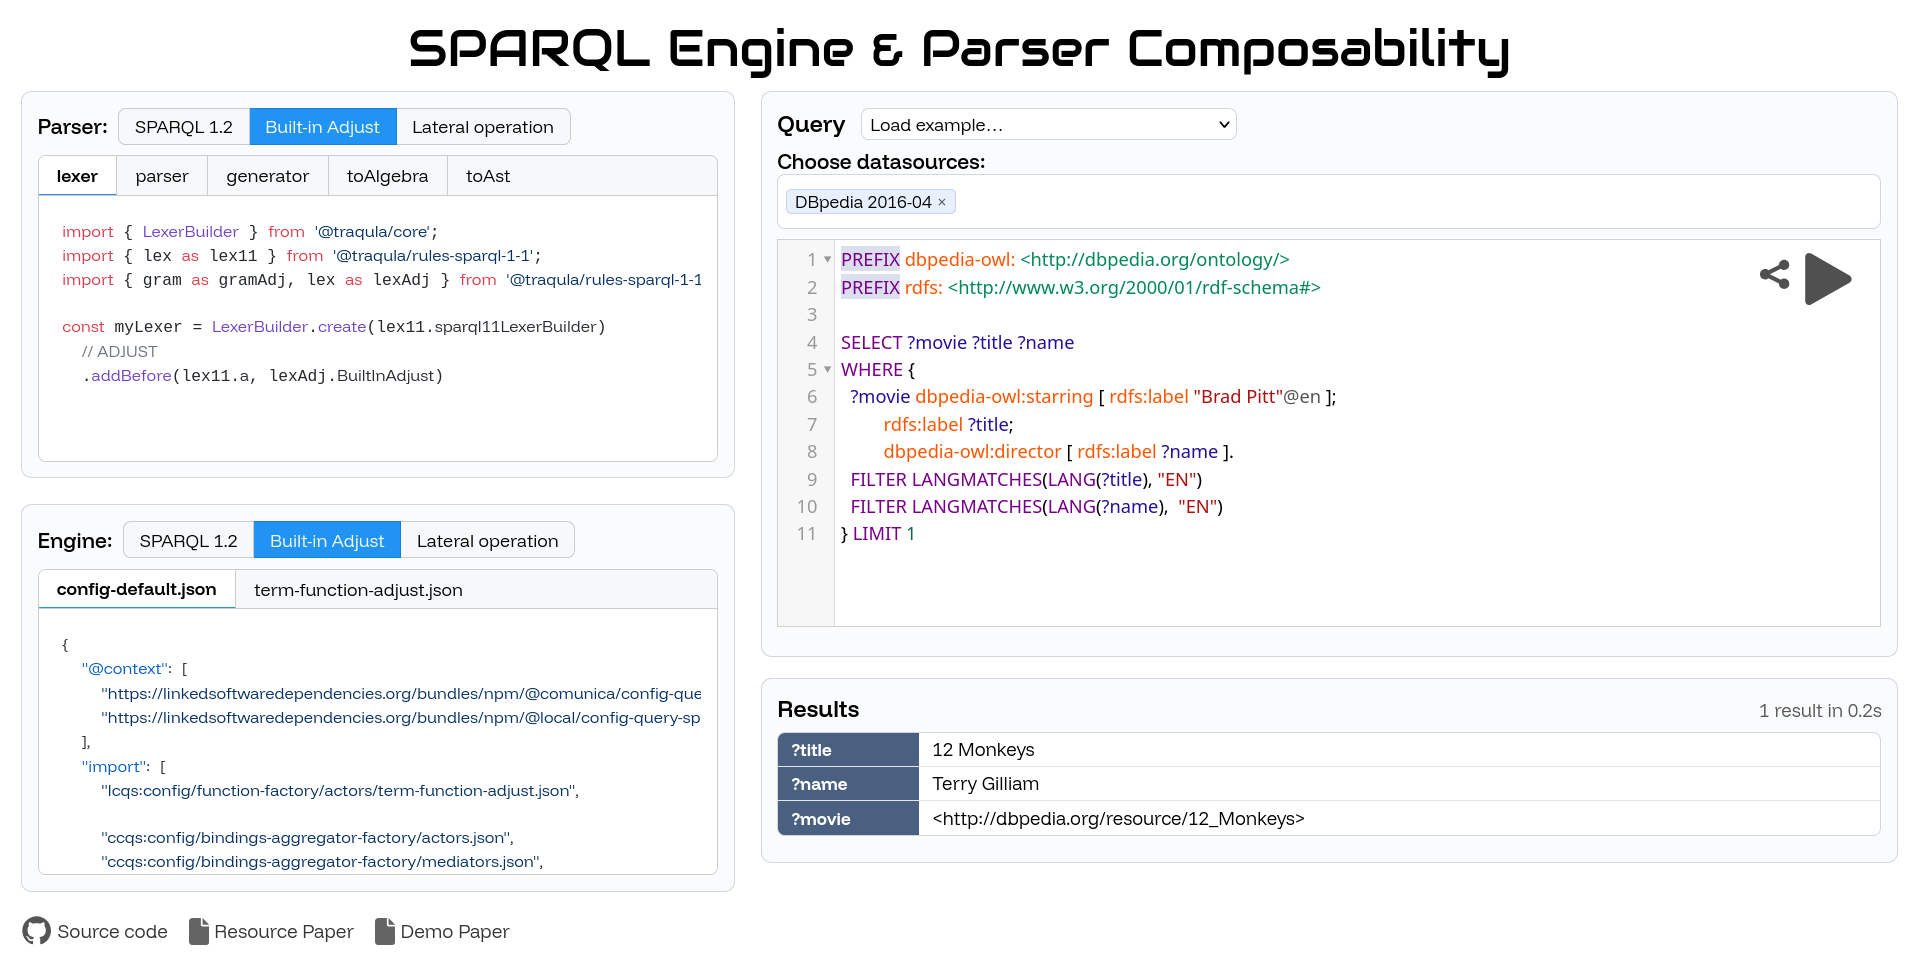
\includegraphics[width=0.9\textwidth, inner]{img/screenshot.png}
        \caption{Screenshot of the web interface demonstrating Traqula and it's integration in Comunica.}
        \label{screenshot}
        \vspace{-12pt}
    \end{figure}

    \begin{credits}
        \subsubsection{\ackname}
        Jitse De Smet is a predoctoral fellow of the Research Foundation -- Flanders (FWO) (1SB8525N).
        Ruben Taelman is a postdoctoral fellow of the Research Foundation -- Flanders (FWO) (1202124N).
    \end{credits}

    \textbf{Disclosure of Interests.} The authors are a subset of the
    developers of both Traqula and Comunica demonstrated in this paper.

%
% ---- Bibliography ----
%
% BibTeX users should specify bibliography style 'splncs04'.
% References will then be sorted and formatted in the correct style.
%
    \bibliographystyle{splncs04}
    \bibliography{references}
\end{document}
